\section{Simulation}
\label{sec:sim}
%%%%%%%%%%%%%%%%%%%%%%%%%%%%%%%%%%%%%%%%%%%%%%%%%%%%%%%%%%%%%%%%%%%%%%%%%%%%%%%%%%%%%%%%%%%%%%%%%%%%%%%%%%%%%%%%%%%%%%%%
A GEANT4 based simulation is performed to asses the sensitivity of the detector to identify 
an emission pattern. Several test emission patterns are used to simulate the propagation of the 
photons through the setup and obtain the hit patterns at the PMTs. The photons detected at the 
PMTs are mapped and put through a statistical test to check the detector's sensitivity towards 
those patterns.

The important geometrical and optical parameters, which are used in the simulation, 
are listed in Table~\ref{tab:OptPar}. The probability for a photon being 
transmitted/reflected at a given surface is 
determined by Fresnel's equations, which include Snell's law for the transmitted light, 
and specular reflection for the reflected light. The boundary surfaces between different media
such as, the LXe--HPFS, HPFS--vacuum and vacuum--PMT, are assumed to be perfectly smooth, 
therefore enabling only specular reflection. 
The photons reaching the PMTs can either be detected, absorbed or reflected from the photocathode 
or from the PMT window. A simplified approach of the above possibilities is considered:
a photon reaching the PMT is considered 30\% probability to be detected (since the PMTs have QE $\geq$ 30\%), 
50\% probability to get absorbed and 20\% probability to get specularly reflected. 
The scintillation light produced in a particular 
event is emitted by a cloud of excimers. This cloud is assumed to have a linear size much smaller than that 
of the optical system. Therefore each event is simulated as a number of photons that are emitted from a point 
in the LXe. The LXe target is much smaller than the mean free path of the source particles, and to 
account for that the events are uniformly generated in the LXe volume.

%%%%%%%%%%%%%%%%%%%%%%%%%%%%%%%%%%%%%%%%%%%%%%%%%%%%%%%%%%%%%%%%%%%%%%%%%%%%%%%%%%%%%%%
\begin{table}[h]
  \centering
  \caption{The parameters used in simulation}
  \label{tab:OptPar}
  \begin{tabular}{|c c||c c|}
  \hline
  Parameter & Value & Parameter & Value \\
  \hline
  LXe absorption length & 100 cm & No. of PMT & 20\\
  %\hline
  LXe scattering length & 35 cm & PMT active area & 22mm $\times$ 22mm\\
  %\hline
  HPFS absorption length & 100 cm & PMT QE & $\geq$ 30\% \\
 % \hline
  HPFS scattering length & $\infty$ & PMT distance from centre & 39 mm\\
 % \hline
  LXe refractive index & 1.61 & LXe bubble radius & 1cm\\
  %\hline
  HPFS refractive index & 1.57 & HPFS shell thickness & 2 cm \\
  Scintillation wavelength & 178 $\pm$ 14 nm & Invar tube diameter & 1 mm\\
  \hline
 \end{tabular}
\end{table}
%%%%%%%%%%%%%%%%%%%%%%%%%%%%%%%%%%%%%%%%%%%%%%%%%%%%%%%%%%%%%%%%%%%%%%%%%%%%%%%%%%%%%%%

In each event the exact number of photons falling on a PMT as well as the exact position 
on the photocathode which the photons hit are not known . The statistical fluctuation 
in the electronic signal generated in a PMT for a certain number of incident photon is 
taken into account. The simulation is performed for both 
ideal photon counting and statistical photon counting. The R8520 PMTs also has  ~20\% probability 
for double photoelectric emission for 178 nm photons, which is also included in the simulation.
Each detected photon on a PMT is assigned a uniformly random position on the PMT surface. 
The direction of this point with respect 
to the center of the LXe sphere is defined as the incident direction of the photon. The direction information 
is then used to calculate the angles between all possible pairs of photon for any event and 
calculate the correlation between all angle pairs.

In order to quantify the anisotropicity of the emission, 
the angle correlation distribution of an anisotropic hit pattern is compared to that of the isotropic 
pattern. A $\chi^2$ test statistics is used where the reduced $\chi^2$ is defined as: 

\begin{equation}
\chi^2/\nu = \frac{1}{\nu} \sum^{\nu}_{i=1} \frac{(O_i - E_i)^2}{E_i},
\label{redchi2}
\end{equation}

where $E_i$ is the pdf of an isotropic emission obtained from a sample of $10^5$ simulated events. 
$O_i$ is the pdf of the anisotropic emission, and $\nu$ is the total number of angle correlation bins 
which is also the degree of freedom. Sixty bins of identical width are used.



%In order to test the emission pattern, the angle correlation distribution of a large sample ($10^5$ events) 
%from isotropic emission is considered as the PDF of the null hypothesis and is compared 
%to that of a number of smaller samples ($10^4$ events) from different types of anisotropic emissions. 
%The reduced $\chi^2$ for each sample is calculated as follows.
%
%\begin{equation}
%\chi^2/\nu = \frac{1}{\nu} \sum^{\nu}_{i=1} \frac{(O_i - E_i)^2}{E_i}
%\label{redchi2}
%\end{equation}
%
%where, $O_i$ is the observed count in the $i^{th}$ angle bin, $E_i$ is the expected count in the $i^{th}$ 
%angle bin and $\nu$ is the total number of angle bins which is also the degree of freedom. In this analysis, 
%60 bins of identical width are used. 


The anisotropic emission patterns used in the analysis are listed 
in Table~\ref{tab:AnisoPattern}. For each emission pattern,  an anisotropic pattern is taken to be embedded 
in an isotropic background. The anisotropic pattern contains  
10\% of the net photons (the fraction of anisotropic signal is denoted by $r_{aniso}$),
while the rest form the isotropic background. For 
multiple beams in a pattern $r_{aniso}$ is split among them 
as mentioned in the Table. The intensity of the beams of photons are of 
Gaussian nature, and their emission direction are 
randomly varied in each event.

%%%%%%%%%%%%%%%%%%%%%%%%%%%%%%%%%%%%%%%%%%%%%%%%%%%%%%%%%%%%%%%%%%%%%%%%%%%%%%%%%%%%%%%
\begin{table}[h]
  \centering
  \caption{Emission patterns. For all patterns $r_{aniso}$ = 0.1 from a 
  total of 50 photon/event.}
  \label{tab:AnisoPattern}
  \begin{tabular}{|c |c |c|cc|cc|}
  \hline
  Pattern no. & No. of beams & type & \multicolumn{2}{c|}{Beam half widths}& \multicolumn{2}{c|}{Signal fractions} \\
 % \hline
  &              &      &  $\sigma_1$ & $\sigma_2$   &  $r_1$ & $r_2$    \\
  \hline
  1 & 1 & & $5^{0}$ & & 1 & \\
  %\hline
   2 & 1 & & $15^{0}$ & & 1 & \\
  %\hline
   3 & 2 & correlated & $5^{0}$ & $5^{0}$ & 0.5 & 0.5  \\
  %\hline
   4 & 2 & correlated & $15^{0}$ & $15^{0}$ & 0.5 & 0.5 \\
  %\hline
   5 & 2 & uncorrelated & $5^{0}$ & $5^{0}$ & 0.5 & 0.5 \\
  %\hline
   6 & 2 & uncorrelated & $5^{0}$ & $10^{0}$ & 0.5 & 0.5 \\
  %\hline
   7 & 2 & uncorrelated & $15^{0}$ & $15^{0}$ & 0.5 & 0.5 \\
  %\hline
   8 & 2 & uncorrelated & $10^{0}$ & $30^{0}$ & 0.5 & 0.5 \\
  %\hline
   9 & 2 & uncorrelated & $10^{0}$ & $30^{0}$ & 0.2 & 0.8 \\
  %\hline
    10 & 2 & uncorrelated & $30^{0}$ & $10^{0}$ & 0.2 & 0.8 \\
  \hline
 \end{tabular}
\end{table}
%%%%%%%%%%%%%%%%%%%%%%%%%%%%%%%%%%%%%%%%%%%%%%%%%%%%%%%%%%%%%%%%%%%%%%%%%%%%%%%%%%%%%%%

A number of data sets generated with different random seeds are 
generated to obtain the 2$\sigma$ fluctuation on <$\chi^2/\nu$>. The <$\chi^2/\nu$> 
and its 2$\sigma$ band for pattern 1 overlaid with the corresponding values 
for an isotropic emission are shown in Fig.~\ref{fig:pattern1}. The <$\chi^2/\nu$> for 
isotropic emission fluctuate around 1 with $\sigma$ = 0.2 which is consistent with 
the expected value of $\frac{1}{\sqrt{30}} \equiv 0.18$ for reduced $\chi^2$ distribution 
with 60 degrees of freedom. The number of events 
$N^{'}$ which is required to achieve <$\chi^2/\nu$> = 2.1, i.e., 5$\sigma$ from the 
band of isotropic emission is set as the pattern distinction criteria. The values of 
$N^{'}$ for all the emission patterns (see Table~\ref{tab:AnisoPattern}) are shown 
in the left panel of Fig.~\ref{fig:convergence}. The values of $N^{'}$, when the fraction of anisotropic 
emission is varied for pattern 1 and pattern 9, are shown in the right panel of Fig.~\ref{fig:convergence}. 

A simulation with two typical sources that emit uniformly in 4$\pi$, a 10 $\mu$Ci $^{137}Cs$ $\gamma$ 
source (662 keV), and a 2.7 $\mu$Ci AmBe neutron source (5 MeV), shows that for an yield of 
50photons/event, it would take about about 0.8 days for 
nuclear recoil (NR) events and 16 days for electron recoil (ER) events to reach a 5$\sigma$ effect. 
Therefore a system that can operate stably for few weeks 
is expected to do reasonable measurements for ER and NR events.


%%%%%%%%%%%%%%%%%%%%%%%%%%%%%%%%%%%%%%%%%%%%%%%%%%%%%%%%%%%%%%%%%%%%%%%%%
\begin{figure}[h]
\centerline{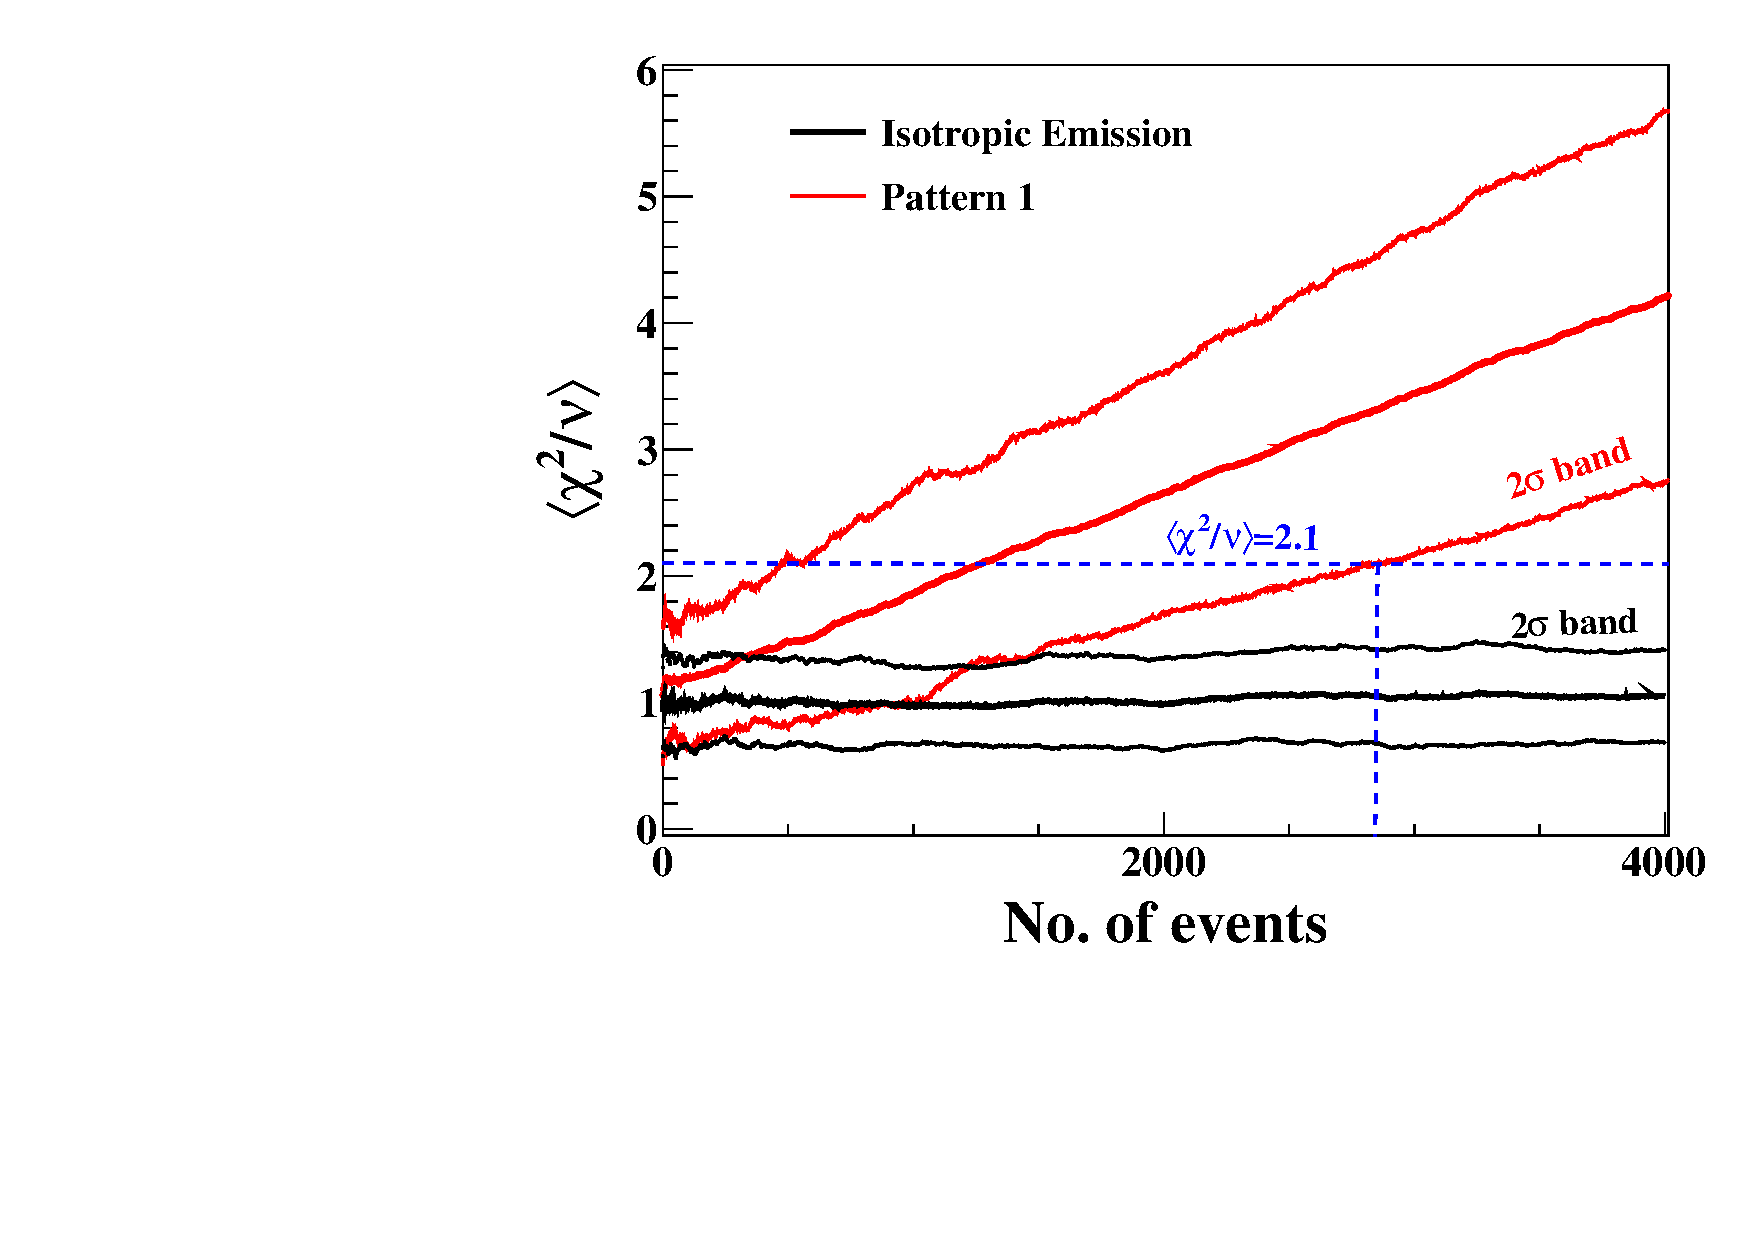
\includegraphics[width=0.5\linewidth]{Pattern1.pdf}}
\caption{<$\chi^2/\nu$> and its $2\sigma$ band for isotropic emission (black) and for pattern 1 (red). 
The number of events needed to discriminate the pattern is defined as that for which 
the $2\sigma$ band crosses <$\chi^2/\nu$> = 2.1, i.e., $5\sigma$ away from the <$\chi^2/\nu$> for isotropy. }
\label{fig:pattern1}
\end{figure}
%%%%%%%%%%%%%%%%%%%%%%%%%%%%%%%%%%%%%%%%%%%%%%%%%%%%%%%%%%%%%%%%%%%%%%%%%%%%

%%%%%%%%%%%%%%%%%%%%%%%%%%%%%%%%%%%%%%%%%%%%%%%%%%%%%%%%%%%%%%%%%%%%%%%%%
\begin{figure}[h]
\centering
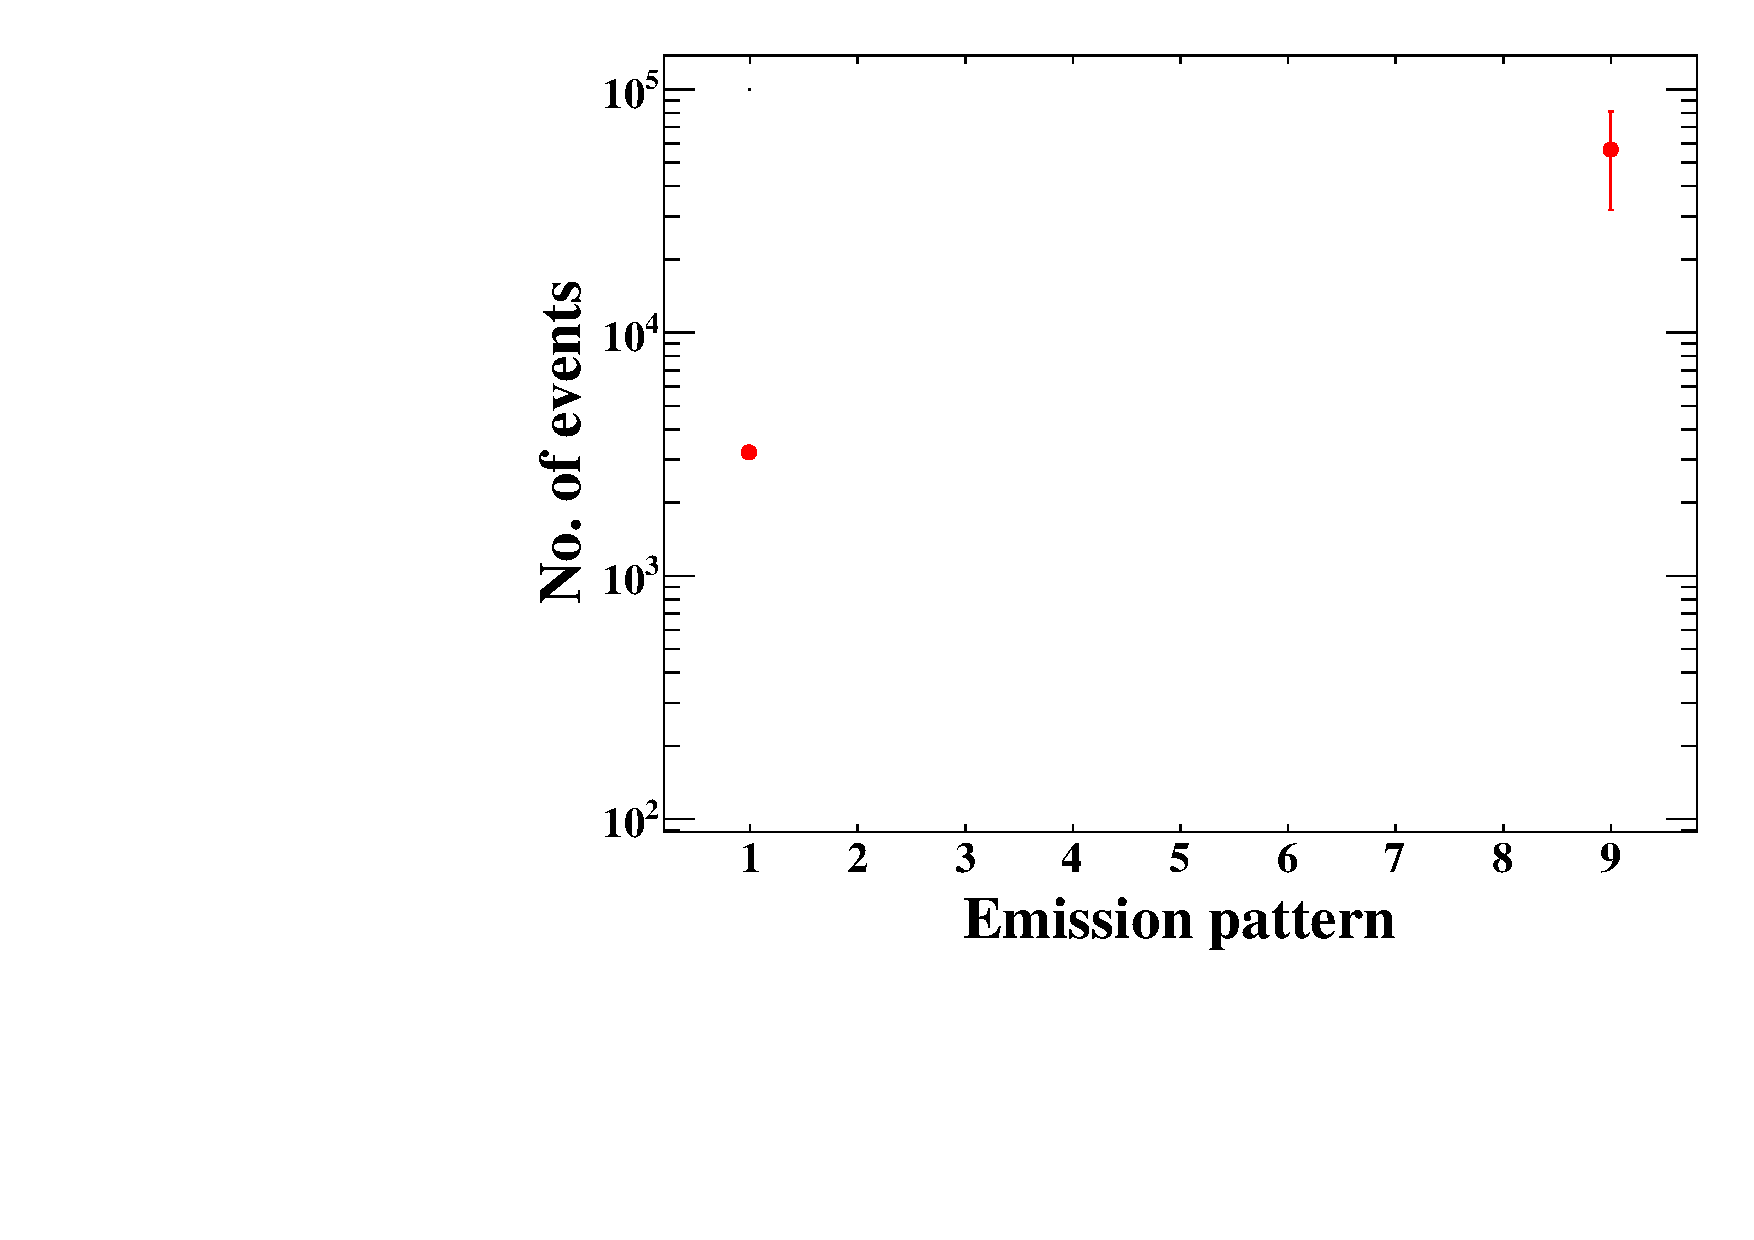
\includegraphics[width=0.45\linewidth]{ConvergenceVsPattern.pdf}
\hspace{0.1cm}
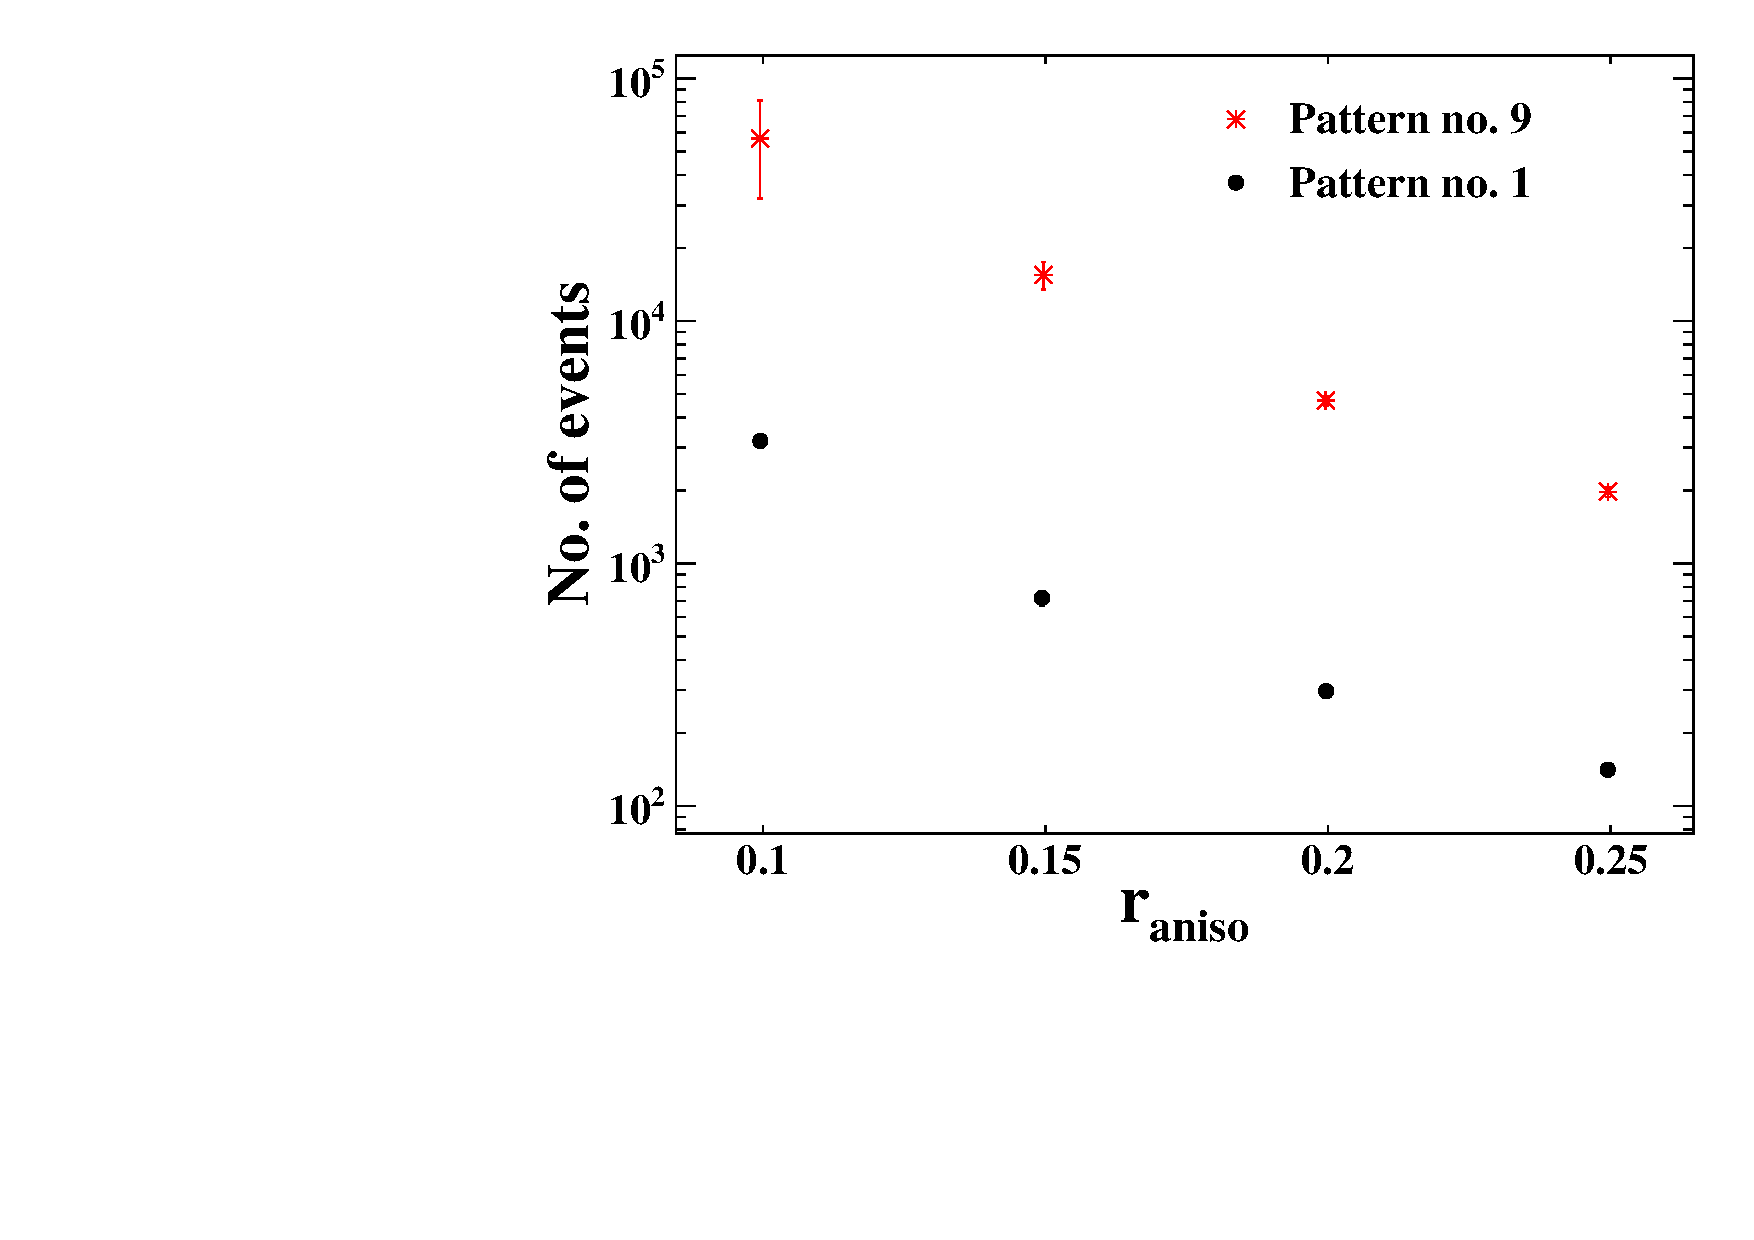
\includegraphics[width=0.45\linewidth]{ConvergenceVsRaniso.pdf}
\caption{(Left) The number of events needed for each emission pattern to cross <$\chi^2/\nu$> = 2.1. Here 
$r_{aniso}$ = 0.1. (Right) The number of events needed for pattern 1 and pattern 9 to cross <$\chi^2/\nu$> = 2.1 
for four different values of $r_{aniso}$.}
\label{fig:convergence}
\end{figure}
%%%%%%%%%%%%%%%%%%%%%%%%%%%%%%%%%%%%%%%%%%%%%%%%%%%%%%%%%%%%%%%%%%%%%%%%%%%%


